% Description: Contains the software state of the art.

\section{Software}
En esta sección, hablaremos de todos los temas relacionados con software que se han investigado para el desarrollo de este proyecto. Se abordarán temas como los firmwares de los controladores de vuelo, las estaciones de control en tierra, los sistemas operativos de las computadoras auxiliares, documentación de ROS 2, visión por computadora, marcadores ArUco, entre otros.

\subsection{FC Firmware}
    La definicion de firmware según ... es \textit{} \cite{}, en el caso de los controladores de vuelo, el firmware es el software que se ejecuta en el controlador de vuelo y se encarga de gestionar los sensores, actuadores y algoritmos de control necesarios para mantener la estabilidad y control del vehículo. Existen varios firmwares de controladores de vuelo disponibles en la actualidad, cada uno con sus propias características y ventajas. En este proyecto, se han investigado dos de los firmwares más populares y ampliamente utilizados en la industria de los drones y vehículos no tripulados: PX4 y ArduPilot.
    \subsubsection{Firmware PX4}
    El firmware PX4 ha sido una pieza fundamental en el desarrollo de sistemas de control de vuelo para drones y vehículos no tripulados, destacándose por su naturaleza de código abierto y su flexibilidad para muchas aplicaciones. Según la documentación oficial, \textit{``PX4 is a powerful open source autopilot flight stack running on the NuttX RTOS''} \cite{px4_docs}. Este sistema es ampliamente reconocido por su arquitectura modular, que permite la integración de nuevos sensores, actuadores y algoritmos de control, facilitando adaptaciones específicas para cumplir con los requisitos de diferentes proyectos \cite{px4_docs}.

    Entre sus características más destacadas, se encuentra su capacidad para soportar una amplia variedad de tipos de vehículos. En este sentido, PX4 \textit{``supports many different vehicle frames/types, including: multicopters, fixed-wing aircraft (planes), VTOLs (hybrid multicopter/fixed-wing), ground vehicles, and underwater vehicles''} \cite{px4_docs}. Esta capacidad de soportar múltiples configuraciones es esencial, ya que permite aplicar el mismo marco de trabajo a diversas plataformas con modificaciones mínimas.

    Además, PX4 es parte integral de un ecosistema más amplio que incluye estaciones de control en tierra como QGroundControl, Mission Planner y hardware específico como Pixhawk. La documentación menciona que \textit{``PX4 is a core part of a broader drone platform that includes the QGroundControl ground station, Pixhawk hardware, and MAVSDK for integration with companion computers, cameras, and other hardware using the MAVLink protocol''} \cite{px4_docs}. Esta integración asegura una comunicación fluida entre los diferentes componentes del sistema, lo cual es crucial para el monitoreo en tiempo real y la planificación de misiones.

    Finalmente, PX4 ofrece \textit{``flexible and powerful flight modes and safety features''} que son vitales para proyectos que requieren maniobras complejas, como el aterrizaje autónomo preciso en estaciones de carga \cite{px4_docs}. Estas funcionalidades avanzadas de control y su capacidad de integrarse con tecnologías de visión por computadora y sensores externos consolidan a PX4 como una herramienta clave en el desarrollo de tecnologías de alta relevancia para vehículos autónomos.
    
    \subsubsection{Firmware ArduPilot}
    ArduPilot, al igual que PX4, es un software de código abierto que se ejecuta en una amplia variedad de hardware, permitiendo la creación y uso de sistemas autónomos de vehículos no tripulados para diferentes aplicaciones. Según la documentación oficial, \textit{“ArduPilot provides a comprehensive suite of tools suitable for almost any vehicle and application. As an open source project, it is constantly evolving based on rapid feedback from a large community of users”} \cite{ardupilot_docs}. Esta flexibilidad y capacidad de adaptación han convertido a ArduPilot en una herramienta esencial para proyectos de automatización y robótica que buscan una solución versátil y robusta.

    Uno de los aspectos más destacados de ArduPilot es que, a diferencia de PX4, éste no fabrica hardware, por lo cual \textit{“ArduPilot firmware works on a wide variety of different hardware to control unmanned vehicles of all types”} \cite{ardupilot_docs}. Esto significa que puede integrarse con distintos tipos de controladores, sensores y dispositivos, transformando prácticamente cualquier máquina móvil en un vehículo autónomo con la simple adición de un paquete de hardware adecuado.

    Como se mencionó anteriormente, el firmware es el código que se ejecuta en el controlador, y la elección del tipo de firmware depende del vehículo y la misión. Como se menciona en la documentación, \textit{“You choose the firmware to match your vehicle and mission: Copter, Plane, Rover, Sub, or Antenna Tracker”} \cite{ardupilot_docs}. Esta versatilidad permite a los desarrolladores seleccionar la configuración más apropiada para sus necesidades específicas, optimizando así el proceso de desarrollo y operación.

    ArduPilot también se complementa con estaciones de control en tierra (GCS), que funcionan como la interfaz entre el usuario y el controlador del vehículo. Una de las herramientas más completas en este ámbito es Mission Planner, descrita como \textit{“a full-featured GCS supported by ArduPilot”}, que ofrece interacción fácil y rápida con el firmware al usuario \cite{ardupilot_docs}.


    Por último, mencionar que tanto PX4 como Ardupilot, tienen funcionalidades similares como la calibraicon de sensores, planificación de misiones, configuración de parámetros, entre otros. Sin embargo, la elección de uno u otro dependerá de las necesidades específicas del proyecto y de la compatibilidad con el \textbf{hardware} disponible.

\subsection{Ground Control Systems}

Las estaciones de control en tierra (GCS, por sus siglas en inglés) son herramientas auxiliares ampliamente utilizadas para la configuración, calibración y monitoreo de drones. Aunque no son el foco principal de este proyecto, desempeñan un papel importante en la preparación del sistema, facilitando la configuración de parámetros, la calibración de sensores y la supervisión durante vuelos de prueba.

Entre las herramientas utilizadas se encuentran QGroundControl y Mission Planner, que destacan por su compatibilidad con los firmwares PX4 y ArduPilot, respectivamente. Estas plataformas proporcionan interfaces intuitivas para ajustar parámetros del vehículo, planificar misiones, y visualizar datos de telemetría en tiempo real. En el contexto de este proyecto, han sido clave para garantizar que el dron esté correctamente configurado antes de integrarse con la estación de carga modular.

A pesar de su utilidad durante las etapas de preparación y pruebas, el sistema propuesto no depende directamente de estas herramientas para su funcionamiento final. La operación autónoma del dron y la estación de carga se basa en la interacción directa entre el firmware, los sistemas de visión, y los controladores de vuelo, sin necesidad de intervención continua desde una estación de control en tierra.

    \begin{figure}[h!]
        \centering
        \begin{minipage}{0.48\textwidth}
            \centering
            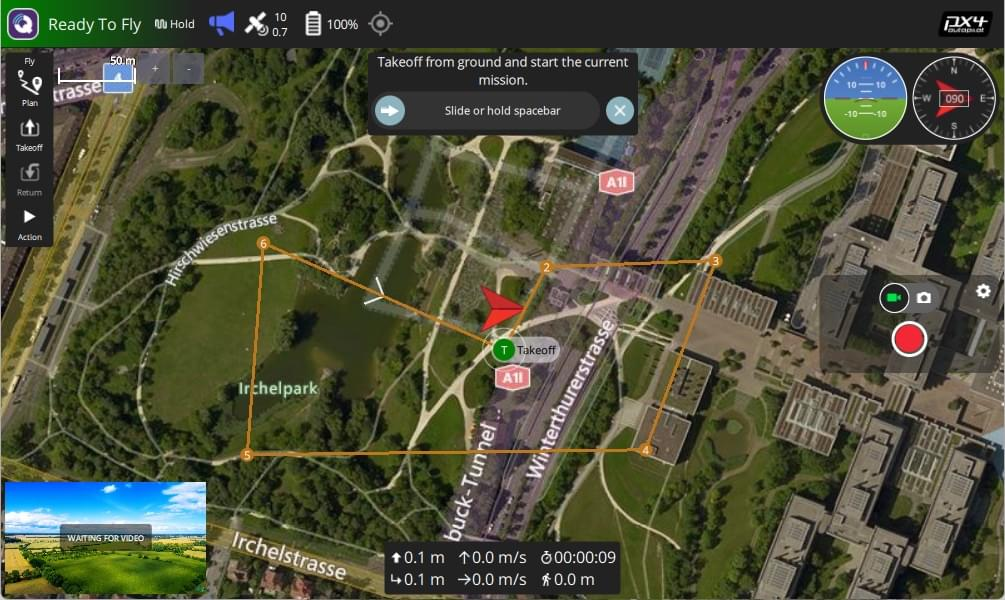
\includegraphics[width=\textwidth]{pictures/qgc_interface.jpg} % Imagen ilustrativa de QGroundControl
            \caption{Interfaz de QGroundControl.}
            \label{fig:qgc}
        \end{minipage}
        \hfill
        \begin{minipage}{0.48\textwidth}
            \centering
            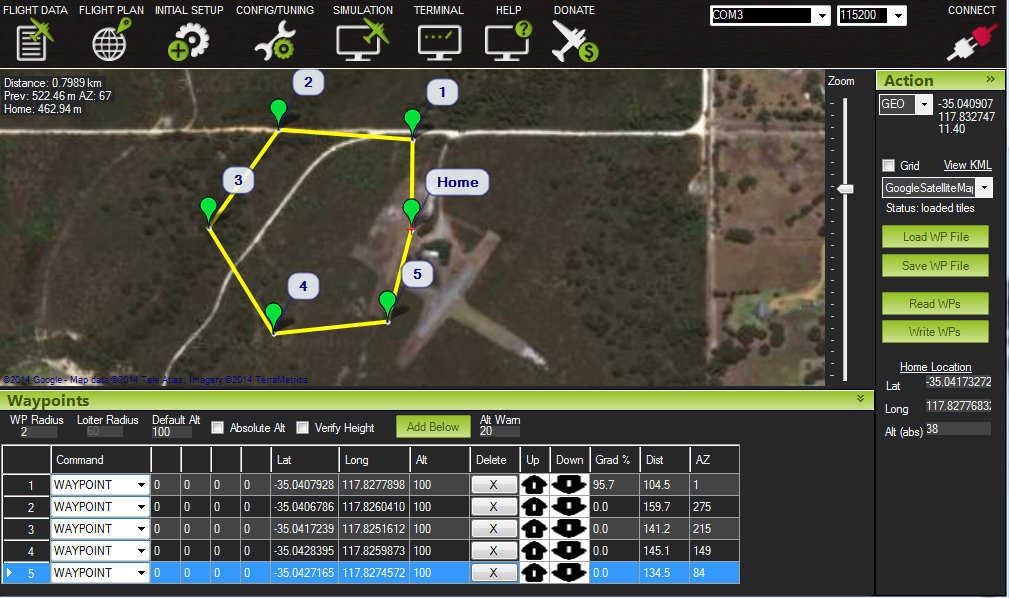
\includegraphics[width=\textwidth]{pictures/mission_planner.jpg} % Imagen ilustrativa de Mission Planner
            \caption{Interfaz de Mission Planner.}
            \label{fig:mission_planner}
        \end{minipage}
        \caption{Estaciones de control en tierra utilizadas durante las etapas de configuración y pruebas.}
        \label{fig:gcs}
    \end{figure}


\subsection{Companion Computer Operative Systems} 
    
    Para poder correr una companion computer se necesita elegir dentro de la multiples opciones de sistemas operativos disponibles, algunos de los más populares son Ubuntu y Raspberry Pi OS. A continuación, se describen las características y ventajas de cada uno de estos sistemas operativos.

    \subsubsection{Ubuntu}

    Ubuntu es un sistema operativo de código abierto basado en Linux que ha ganado popularidad por su estabilidad y amplia comunidad de soporte, es importante saber que dentro de Ubuntu y sus versiones, las versiones pares son las que tienen mayor estabilidad. Según la documentación oficial de Ubuntu, este sistema es \textit{“designed for security, reliability, and ease of use”} \cite{ubuntu_docs}. En el contexto de los companion computers para drones y otros vehículos autónomos, Ubuntu se utiliza frecuentemente debido a su compatibilidad con herramientas de robótica como ROS (Robot Operating System), lo que facilita la integración y desarrollo de software avanzado de control y automatización.

    Ubuntu ofrece soporte para arquitecturas ARM, lo que permite su instalación y ejecución en dispositivos como la Raspberry Pi 4 y 5. Esta capacidad es fundamental para proyectos que requieren procesamiento local eficiente, manejo de datos de sensores y comunicación en tiempo real. Adicionalmente, la flexibilidad de Ubuntu permite la personalización de su entorno para adaptarse a las necesidades específicas del proyecto, ya sea para ejecutar nodos de control de vuelo o procesamiento de imágenes en tiempo real.


    \subsubsection{Raspberry Pi OS}

    Raspberry Pi OS, es el sistema operativo oficial desarrollado y optimizado para dispositivos Raspberry Pi. La documentación de Raspberry Pi OS lo describe como \textit{“a Debian-based operating system specifically tuned for the Raspberry Pi hardware”} \cite{raspbian_docs}. Su principal ventaja es su optimización para el hardware de Raspberry Pi, lo que garantiza un rendimiento óptimo y un uso eficiente de los recursos disponibles.

    Raspbian incluye una serie de herramientas preinstaladas que facilitan el desarrollo y prototipado, haciendo que sea una opción preferida para proyectos educativos y de investigación. La compatibilidad con Python y otras bibliotecas de programación facilita la implementación de scripts y software necesarios para el control de drones y otras aplicaciones robóticas.

    En comparación con otros sistemas operativos, Raspbian es ligero y permite un arranque rápido, lo cual es beneficioso en escenarios donde se requiere un inicio rápido del sistema. Además, la comunidad activa de usuarios de Raspberry Pi proporciona recursos y asistencia que resultan invaluables para la resolución de problemas y la optimización del software.


\subsection{ROS2 Distributions}
    Las distribuciones de ROS 2 (Robot Operating System 2) proporcionan entornos estandarizados para el desarrollo de aplicaciones robóticas, cada una adaptada a diferentes necesidades y capacidades de hardware. Una de las ventajas de ROS 2 es su capacidad para facilitar la comunicación entre distribuciones mediante el uso de topics, lo que permite que nodos en distintas versiones de ROS 2 se comuniquen y colaboren de manera efectiva en un mismo proyecto \cite{ros_docs}. En la siguiente sección se abordarán más detalles sobre el funcionamiento general de ROS 2 y su importancia en proyectos de robótica.

    En el contexto de companion computers como la Raspberry Pi, las distribuciones específicas de ROS 2 se eligen basándose en la versión de hardware y la compatibilidad de software. La Raspberry Pi 4, por ejemplo, es adecuada para ejecutar la distribución ROS 2 Humble \cite{raspberry_docs}, mientras que la Raspberry Pi 5 puede correr la distribución más reciente, ROS 2 Jazzy Jalisco \cite{ros_docs}. A continuación, se describen las principales características de cada distribución y algunas diferencias importantes.
    \subsubsection{Distribución Humble}

    La distribución ROS 2 Humble es conocida por su estabilidad y soporte a largo plazo (LTS), lo que la convierte en una opción popular para proyectos que requieren fiabilidad y consistencia en el tiempo. Esta versión es ideal para proyectos que utilizan hardware como la Raspberry Pi 4, ya que está optimizada para correr de manera eficiente en dispositivos con arquitecturas ARM \cite{humble_documentation}.

    Características principales de ROS 2 Humble:

    Soporte a largo plazo (LTS), garantizando actualizaciones y soporte extendido.
    Mayor estabilidad en la comunicación entre nodos.
    Compatibilidad con una amplia gama de paquetes y bibliotecas de ROS.
    Recomendado para proyectos de investigación y aplicaciones de largo plazo.

    \subsubsection{Distribución Jazzy}

    La distribución ROS 2 Jazzy Jalisco es una de las más recientes y está diseñada para aprovechar las capacidades avanzadas del hardware más moderno, como la Raspberry Pi 5. Esta versión incluye mejoras en rendimiento y nuevas funcionalidades que facilitan el desarrollo de aplicaciones robóticas más complejas y eficientes \cite{jazzy_documentation}.

    Características principales de ROS 2 Jazzy Jalisco:

    Introducción de características experimentales y optimizaciones de rendimiento.
    Mejoras en la latencia y el manejo de la comunicación entre nodos.
    Integración mejorada con nuevas herramientas de simulación y depuración.
    Adecuado para desarrolladores que buscan utilizar las últimas funcionalidades de ROS 2 en proyectos avanzados.
    Ambas distribuciones comparten la capacidad de usar el middleware DDS (Data Distribution Service) para la comunicación entre nodos, permitiendo la creación de sistemas distribuidos y escalables. La elección entre ROS 2 Humble y Jazzy Jalisco dependerá de las especificaciones de hardware disponibles y las necesidades específicas del proyecto.

    \begin{figure}[h!]
        \centering
        \begin{minipage}{0.45\textwidth}
            \centering
            
\includegraphics[width=0.5\textwidth]{pictures/humble_logo.png}
            \caption{ROS 2 Humble}
            \label{fig:imagen1}
        \end{minipage}
        \hfill
        \begin{minipage}{0.45\textwidth}
            \centering
            
\includegraphics[width=0.6\textwidth]{pictures/jazzy_logo.png}
            \caption{ROS 2 Jazzy Jalisco}
            \label{fig:imagen2}
        \end{minipage}
    \end{figure}

\subsection{ROS2 Documentation}
    ROS 2 (Robot Operating System 2) es un conjunto de bibliotecas y herramientas que permiten a los desarrolladores crear aplicaciones de robótica. Es una evolución de ROS 1, diseñada para abordar limitaciones en términos de escalabilidad, seguridad y soporte a sistemas en tiempo real. ROS 2 ofrece un marco de trabajo robusto que facilita la implementación de sistemas distribuidos y permite la comunicación entre múltiples nodos a través de una arquitectura basada en el middleware DDS (Data Distribution Service) \cite{ros_docs}. A continuación, se detallan los beneficios y la estructura de ROS 2.

    \subsubsection{Benefits of ROS2}

    ROS 2 introduce mejoras significativas que lo hacen más adecuado para aplicaciones avanzadas de robótica. Entre los principales beneficios se encuentran:

    \begin{itemize} \item Multithreading y manejo en tiempo real: ROS 2 permite la ejecución de múltiples nodos en paralelo, lo que mejora el rendimiento en aplicaciones complejas. \item Comunicación mediante topics, nodos y servicios: Facilita la creación de sistemas distribuidos donde los nodos se comunican de forma eficiente. \item Archivos de lanzamiento (launchfiles): Simplifican la ejecución de múltiples nodos y configuraciones mediante un solo archivo. \item Baja latencia y comunicación rápida: La arquitectura basada en DDS proporciona una comunicación confiable y de baja latencia, esencial para aplicaciones críticas. \item Diferentes tipos de mensajes: Soporte para mensajes personalizados y definidos por el usuario. \end{itemize}

    \begin{table}[h!]
    \centering
    \caption{Beneficios clave de ROS 2}
    \begin{tabular}{|l|p{10cm}|}
    \hline
    \textbf{Beneficio} & \textbf{Descripción} \\
    \hline
    Multithreading & Permite la ejecución de nodos en paralelo, optimizando el rendimiento \\
    \hline
    Uso de topics & Comunicación asincrónica entre nodos para el intercambio de datos \\
    \hline
    Nodos y servicios & Los nodos son unidades de ejecución que interactúan mediante servicios y topics \\
    \hline
    Archivos de lanzamiento (launchfiles) & Permiten la configuración y ejecución de múltiples nodos simultáneamente \\
    \hline
    Comunicación rápida & Basada en DDS, proporciona comunicación de baja latencia \\
    \hline
    Mensajes personalizados & Soporte para definir y usar mensajes específicos para aplicaciones personalizadas \\
    \hline
    \end{tabular}
    \label{table}
    \end{table}

    \subsubsection{ROS2 Architecture}

    Dentro de la documentación oficial de ROS 2 se habla de que un aspecto central de esta arquitectura son los nodos, que actúan como las unidades básicas de procesamiento en un sistema de ROS 2. Los nodos se comunican entre sí mediante topics, que permiten un intercambio de información asincrónico y eficiente.

    Los mensajes en ROS 2 definen la estructura de los datos que se transmiten a través de topics. Estos mensajes pueden ser de tipos predefinidos o personalizados, adaptándose a las necesidades de la aplicación. Los servicios, por otro lado, permiten una comunicación sincrónica entre nodos, donde un nodo solicita una acción específica y otro nodo responde con el resultado.

    Los archivos de lanzamiento, o launchfiles, son documentos que permiten ejecutar múltiples nodos y configurar parámetros de forma simultánea. Facilitan la gestión de sistemas complejos, ya que centralizan la configuración en un solo archivo, lo que simplifica la puesta en marcha de aplicaciones robóticas \cite{ros_docs}.

    Finalmente, ROS 2 admite la configuración y uso de parámetros, que son variables accesibles desde los nodos para ajustar comportamientos en tiempo de ejecución sin necesidad de recompilar el código.

    \begin{figure}[h!] 
    \centering 
    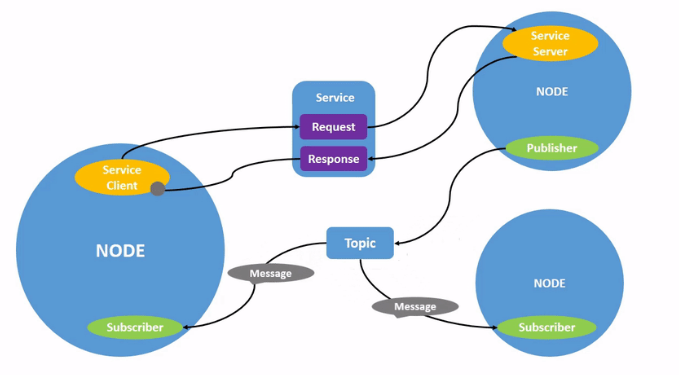
\includegraphics[width=0.8\textwidth]{pictures/ros2_arch.png} % Imagen ilustrativa de la estructura de ROS 2 
    \caption{Estructura de ROS 2, mostrando la interacción de nodos, topics, servicios y launchfiles.}
    \label{fig} 
    \end{figure}

\subsection{Computer Vision}
    

    La visión por computadora es un campo de la programación que permite a los sistemas interpretar y procesar información visual del mundo que los rodea. Es esencial para aplicaciones que requieren el análisis de imágenes y videos en tiempo real, como la navegación autónoma de vehículos, detección de objetos, inteligencia artificial, etc.

    \subsubsection{OpenCV Library}

    OpenCV (Open Source Computer Vision Library) es una biblioteca de código abierto ampliamente utilizada en la industria y en la investigación académica para el desarrollo de aplicaciones de visión por computadora. De acuerdo con la documentación oficial, OpenCV es \textit{“an open-source computer vision and machine learning software library containing more than 2500 optimized algorithms”} \cite{opencv_docs}. Esta biblioteca proporciona herramientas para tareas como el procesamiento de imágenes, reconocimiento de objetos, seguimiento de movimiento, entre otras, y es compatible con múltiples lenguajes de programación como Python, C++ y más.

    OpenCV es conocida por su flexibilidad y facilidad de uso, lo que la hace popular tanto entre principiantes como entre expertos en el área de la visión por computadora. La biblioteca incluye funciones de alto rendimiento que pueden ser ejecutadas en tiempo real, haciendo que sea una opción ideal para proyectos de robótica y sistemas autónomos \cite{arevalo2004}.

    \subsubsection{Camera Calibration}

    La calibración de cámaras es un proceso crucial en la visión por computadora, necesario para corregir distorsiones inherentes a las lentes de las cámaras y obtener mediciones precisas del entorno. Este proceso implica la obtención de parámetros intrínsecos y extrínsecos que permiten mapear las coordenadas 2D de una imagen a coordenadas 3D en el mundo real.

    \begin{figure}[h!] 
    \centering 
    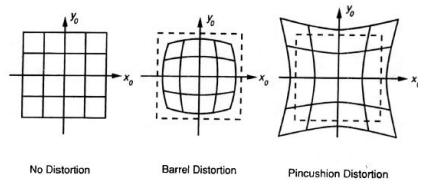
\includegraphics[width=0.6\textwidth]{pictures/distortions.png} % Imagen de distorciones de barril y cojín inherentes a las cámaras 
    \caption{Tipos de distorciones de cámaras}
    \label{fig} 
    \end{figure}

    Según la documentación de OpenCV, \textit{“Camera calibration is the process of estimating the parameters of the lens and the image sensor of an imaging device”} \cite{opencv_calib3d}. OpenCV proporciona herramientas y funciones que permiten realizar este proceso de manera eficiente mediante la detección de patrones en imágenes, como tableros de ajedrez o círculos.

    El flujo típico de calibración de una cámara con OpenCV incluye capturar imágenes de un patrón conocido, identificar los puntos de interés en cada imagen y utilizar algoritmos de optimización para calcular los parámetros de la cámara. Estos parámetros incluyen la distancia focal, el punto principal, y los coeficientes de distorsión radial y tangencial \cite{opencv_tutorial_calib}.

    Además, se pueden utilizar los resultados de la calibración para corregir la distorsión en imágenes y videos, mejorando así la precisión de las aplicaciones de visión por computadora y el uso para calcular la pose o posiciónes de algunos objetos de interés. El uso de una cámara calibrada es fundamental en proyectos que requieren un análisis espacial preciso, como la navegación autónoma de robots y drones.

    \begin{figure}[h!] 
    \centering 
    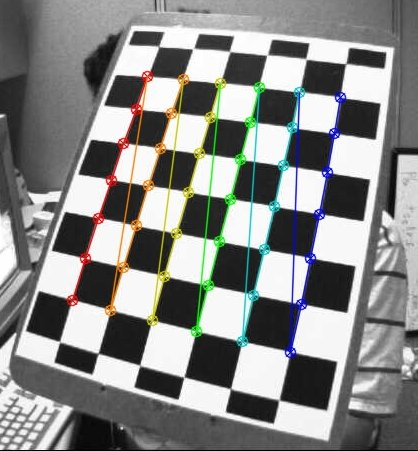
\includegraphics[width=0.4\textwidth]{pictures/calib_pattern.jpg} % Imagen ilustrativa de un tablero de ajedrez para calibración de cámaras 
    \caption{Patrón de tablero de ajedrez utilizado en la calibración de cámaras con OpenCV.} \label{fig} 
    \end{figure}

\subsection{What is an ArUco?}
    ArUco, cuyo nombre proviene de la combinación de "Artificial" y "Uco" (por la Universidad de Córdoba, donde se desarrolló), es una biblioteca de código abierto ampliamente reconocida en el ámbito de la visión por computadora para la detección de marcadores fiduciales en imágenes. Esta tecnología es fundamental para la estimación de la pose de la cámara con respecto a los marcadores cuando la cámara ha sido previamente calibrada. De acuerdo con la documentación, \textit{“ArUco is an OpenSource library for detecting squared fiducial markers in images”} \cite{aruco_docs}. La detección de estos marcadores es crucial en aplicaciones que requieren una estimación precisa de la posición y orientación de objetos en el espacio tridimensional.

    \subsubsection{Historia de los Marcadores Aruco}

    Los marcadores ArUco se originaron como una solución para superar las limitaciones de otras tecnologías de detección de patrones, colores o figuras. El objetivo era desarrollar una técnica que proporcionara alta fiabilidad incluso bajo oclusiones parciales y condiciones de iluminación variables. Los primeros estudios se centraron en la generación automática de marcadores con un diseño que asegurara su unicidad y facilidad de detección. Estos marcadores están compuestos por un patrón binario rodeado de un borde negro, lo que mejora su visibilidad y robustez en diferentes condiciones de iluminación \cite{aruco_docs}.

    \begin{figure}[h!] 
    \centering 
    %\includegraphics[width=0.8\textwidth]{example_image.jpg} % Ejemplo de marcadores ArUco 
    \caption{ArUco example} 
    \label{fig} 
    \end{figure}

    \subsubsection{Aplicaciones Comunes}

    Los marcadores ArUco se utilizan en una variedad de aplicaciones, que incluyen la calibración de cámaras, la realidad aumentada, y el control y navegación de robots y drones. Una de las ventajas de usar ArUco es su capacidad para actuar como puntos de referencia en entornos 3D, permitiendo a los sistemas de visión por computadora calcular la pose de la cámara. Según la documentación, \textit{“Markers can be used as 3D landmarks for camera pose estimation”} \cite{aruco_docs_pdf}. Esta característica hace que los marcadores sean esenciales en sistemas de seguimiento y posicionamiento donde la precisión es crítica.

    \begin{figure}[h!] 
    \centering 
    %\includegraphics[width=0.8\textwidth]{example_image.jpg} % Ejemplo de pose de un marcador ArUco siendo detectada 
    \caption{ArUco pose estimation} 
    \label{fig} 
    \end{figure}

    \subsubsection{Formatos de Marcadores}

    Los marcadores ArUco están compuestos por un borde negro externo y una región interna que codifica un patrón binario único. Dependiendo del diccionario que se esté utilizando, el número de bits en el marcador varía, lo que afecta la probabilidad de confusión con otros marcadores y la distancia de detección. Una mayor resolución de los marcadores permite que estos se detecten desde distancias más lejanas, pero puede requerir mayor procesamiento \cite{aruco_docs}.

    La biblioteca ArUco también soporta la creación de diccionarios personalizados, lo que permite a los desarrolladores adaptar los marcadores a las necesidades específicas de sus proyectos. \textit{“The design of a dictionary is important since the idea is that their markers should be as different as possible to avoid confusions”} \cite{aruco_docs_pdf}. Esta flexibilidad es especialmente útil en proyectos donde es crucial mantener la unicidad y fiabilidad de la detección de marcadores en entornos complejos.

    \begin{figure}[h!] 
    \centering 
    %\includegraphics[width=0.8\textwidth]{example_image.jpg} % Ejemplo de marcador ArUco con su formato binario 
    \caption{Imagen explicación de bits en ArUco} 
    \label{fig} 
    \end{figure}

\subsection{Aruco vs Embedded Aruco}
    Los marcadores ArUco y los marcadores Embedded ArUco (e-ArUco) son tecnologías utilizadas en visión por computadora para tareas de detección y estimación de pose. Aunque ambos comparten una base común en cuanto a su diseño y algoritmos de detección, tienen diferencias importantes que los hacen adecuados para distintas aplicaciones, especialmente en el contexto de operaciones de alta precisión y entornos desafiantes.

    \subsubsection{Diferencias Principales}

    La principal diferencia entre los marcadores ArUco tradicionales y los marcadores Embedded ArUco radica en la optimización de estos últimos para detecciones de alta precisión en un rango amplio de distancias. Según Khazetdinov et al. (2021), \textit{“a new type of fiducial marker called embedded ArUco (e-ArUco) was developed specially for a task of robust marker detection for a wide range of distances”} \cite{khazetdinov2021}. Los e-ArUco están diseñados para mantener su detectabilidad y precisión en escenarios donde los marcadores ArUco estándar podrían no ser tan efectivos, como cuando se requiere una precisión milimétrica en aplicaciones de aterrizaje de UAVs.

    Otra diferencia significativa es que los marcadores e-ArUco están diseñados para mejorar la robustez de la detección, minimizando los errores que podrían surgir por condiciones de iluminación cambiantes y oclusiones parciales. Estos marcadores se basan en los algoritmos de detección de ArUco, lo que permite su implementación sin cambios sustanciales en los sistemas existentes basados en ArUco \cite{khazetdinov2021}.

    \subsubsection{Casos de Uso}

    Los marcadores ArUco tradicionales como se mencionó en la sección anterior, se utilizan comúnmente en aplicaciones de realidad aumentada, estimacion de poses y navegación de robots y drones. Estos marcadores son versátiles y se pueden adaptar a diversas aplicaciones que no requieren una precisión extrema, siendo ideales para proyectos de investigación y desarrollo.

    Por otro lado, los marcadores Embedded ArUco (e-ArUco) están específicamente diseñados para situaciones donde la precisión es más crítica. Un ejemplo destacado es el uso en el aterrizaje de UAVs (vehículos aéreos no tripulados), donde se necesita una detección precisa y confiable a diferentes distancias. En un estudio realizado por Khazetdinov et al., tuvo como resultado \textit{“an average landing accuracy was 2.03 cm with a standard deviation of 1.53 cm”} al usar marcadores e-ArUco y un algoritmo de aterrizaje implementado en ROS y probado en el simulador Gazebo \cite{khazetdinov2021}. Esta capacidad hace que los e-ArUco sean ideales para entornos donde se requiere una precisión milimétrica, como en operaciones de aterrizaje autónomo de alta precisión.

    \begin{figure}[h!]
        \centering
        \begin{minipage}{0.3\textwidth}
            \centering
            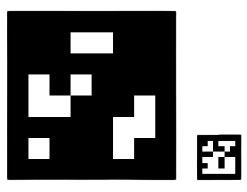
\includegraphics[width=0.65\textwidth]{pictures/pose_1.png}
            \caption{Generación de ArUco Grande / Chico}
            \label{fig:imagen1}
        \end{minipage}
        \hfill
        \begin{minipage}{0.3\textwidth}
            \centering
            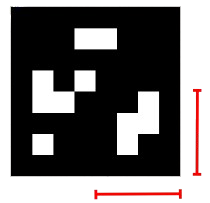
\includegraphics[width=0.55\textwidth]{pictures/pose_2.png}
            \caption{Cálculo del centro del ArUco Grande}
            \label{fig:imagen2}
        \end{minipage}
        \hfill
        \begin{minipage}{0.3\textwidth}
            \centering
            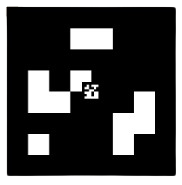
\includegraphics[width=0.5\textwidth]{pictures/pose_3.png}
            \caption{Sobreposición del ArUco Chico en el centro del Grande}
            \label{fig:imagen2}
        \end{minipage}
    \end{figure}

\subsection{Aruco Detection}
    La detección de marcadores ArUco es un proceso esencial en la visión por computadora que permite la identificación y estimación de la pose de los marcadores en imágenes. La siguiente sección detalla los algoritmos de detección, la implementación en OpenCV y los parámetros que afectan la precisión de la detección.

    \subsubsection{Algoritmos de Detección}

    La detección de los marcadores ArUco se basa en algoritmos de visión por computadora que identifican contornos y patrones específicos en las imágenes. Según la documentación de OpenCV, el proceso de detección comienza con la identificación de cuadrados en la imagen y la verificación de si estos contienen un patrón binario válido correspondiente a un marcador ArUco \cite{opencv_docs_aruco}. El algoritmo implementado en OpenCV utiliza la segmentación de contornos y la detección de bordes para encontrar regiones cuadradas que luego se comprueban para determinar si coinciden con los patrones en el diccionario de ArUco.

    Una vez que se identifica un marcador, el algoritmo calcula la pose de la cámara en relación con el marcador utilizando la proyección inversa. Este proceso es particularmente importante en aplicaciones donde se necesita calcular la posición y orientación de la cámara para la navegación y el control de robots y drones.

    \subsubsection{Implementación en OpenCV}

    OpenCV ofrece una implementación robusta para la detección de marcadores ArUco a través del módulo \texttt{cv::aruco}. La función principal para la detección es \texttt{cv::aruco::detectMarkers}, que se encarga de identificar los marcadores en una imagen y devolver sus esquinas y los IDs correspondientes. La documentación de OpenCV resalta que \textit{“the function detects the markers and returns their IDs and corner positions in the image”} \cite{opencv_tutorial_aruco}.

    El siguiente ejemplo muestra cómo usar OpenCV para detectar marcadores ArUco en Python:

    \begin{verbatim} import cv2 import cv2.aruco as aruco

    Cargar la imagen
    image = cv2.imread('image_path.jpg')

    Definir el diccionario de ArUco
    aruco_dict = aruco.Dictionary_get(aruco.DICT_6X6_250)

    Detectar los marcadores
    corners, ids, _ = aruco.detectMarkers(image, aruco_dict)

    Dibujar los marcadores detectados
    if ids is not None: aruco.drawDetectedMarkers(image, corners, ids) \end{verbatim}

    Este código permite la detección y visualización de los marcadores ArUco en una imagen de una forma muy simple, devolviendo las posiciones de las esquinas y los IDs de los marcadores detectados.

    \subsubsection{Parámetros de Precisión}

    La precisión de la detección de marcadores ArUco depende de varios factores, incluidos la calidad de la imagen, el tamaño del marcador, y los parámetros de calibración de la cámara. Según la documentación de OpenCV, la calibración precisa de la cámara es fundamental para minimizar los errores en la estimación de la pose \cite{opencv_docs_aruco}. Entre los parámetros que afectan la detección se encuentran:

    \begin{itemize} \item \textbf{Distorsión de la lente}: La corrección de la distorsión de la lente mejora la precisión de la detección. \item \textbf{Resolución del marcador}: Marcadores con mayor resolución permiten una detección más precisa a distancias más largas, pero requieren más recursos de procesamiento. \item \textbf{Iluminación y contraste}: La detección puede verse afectada por condiciones de iluminación variables, por lo que es importante que la imagen tenga un buen contraste entre el marcador y el fondo. \end{itemize}

    \begin{figure}[h!] 
        \centering 
        %\includegraphics[width=0.8\textwidth]{example_image.jpg} % Ejemplo de detección de marcadores ArUco en una imagen 
        \caption{Detección de marcadores ArUco con OpenCV mostrando los IDs y las esquinas detectadas.} 
        \label{fig} 
    \end{figure}

\subsection{Comunicación ROS2 - Pixhawk}
    La comunicación entre ROS 2 y Pixhawk se basa en el uso de MAVLink, un protocolo ligero que permite la transferencia bidireccional de datos entre el controlador de vuelo y una computadora auxiliar (companion computer). Esta integración es crucial para enviar comandos de vuelo en tiempo real y monitorizar el estado del dron.
    
        \subsubsection{Protocolo MAVLink}
        MAVLink (Micro Air Vehicle Link) es un protocolo de comunicación de alto rendimiento diseñado para sistemas de vehículos no tripulados. Según la documentación oficial, \textit{“MAVLink is a very lightweight, header-only message marshalling library for micro air vehicles”} \cite{mavlink_docs}. Este protocolo utiliza un sistema basado en paquetes de mensajes que facilita la transmisión de datos entre la estación de control y el vehículo no tripulado.
    
        Los mensajes de MAVLink están estructurados en comandos específicos que permiten controlar varios aspectos del vuelo y la telemetría, incluyendo parámetros como la posición, velocidad, estado de la batería, y comandos de control de vuelo. Cada mensaje está identificado por un ID único, lo que facilita su procesamiento y permite una comunicación eficiente en tiempo real.
    
        \subsubsection{Opciones de Integración de MAVLink en ROS 2}
        Para facilitar la integración de MAVLink con ROS 2, existen varias opciones de comunicación que permiten enviar y recibir datos entre una computadora auxiliar y el controlador de vuelo Pixhawk. Las dos soluciones más populares son MAVROS y Micro XRCE-DDS.
    
            \paragraph{MAVROS}
            es un conjunto de nodos ROS que actúa como una interfaz entre ROS y MAVLink, permitiendo que ROS se comunique con Pixhawk mediante topics y servicios. MAVROS permite la publicación y suscripción de mensajes de MAVLink a través de topics en ROS, facilitando la ejecución de comandos de vuelo, obtención de datos de telemetría y control de misiones.
    
            MAVROS implementa una serie de topics predefinidos en ROS, tales como:
            \begin{itemize}
                \item \texttt{/mavros/setpoint\_position/local}: Para establecer puntos de referencia de posición.
                \item \texttt{/mavros/state}: Proporciona el estado actual del dron, incluyendo el modo de vuelo y si el vehículo está armado.
                \item \texttt{/mavros/imu/data}: Datos de IMU para el monitoreo de la orientación y aceleración.
            \end{itemize}
            
            Con MAVROS, los desarrolladores pueden enviar comandos de control, como armar el dron, cambiar el modo de vuelo, o establecer puntos de referencia para la navegación autónoma. Esto se realiza publicando mensajes en los topics adecuados y ajustando parámetros en tiempo real mediante la interfaz de MAVLink \cite{px4_ros2}.
    
            \paragraph{Micro XRCE-DDS}
            es una implementación ligera del DDS (Data Distribution Service) que permite la comunicación entre ROS 2 y Pixhawk de forma eficiente en sistemas con limitaciones de recursos. Esta opción es útil en contextos donde el tamaño y rendimiento del sistema son cruciales, como en drones pequeños o con hardware de procesamiento limitado.
    
            Con Micro XRCE-DDS, ROS 2 puede comunicarse directamente con PX4 utilizando el middleware DDS. Esto permite la creación de un sistema distribuido y escalable, en el cual los nodos de ROS 2 pueden enviar y recibir mensajes MAVLink a través de topics DDS, de manera similar a MAVROS, pero con una carga de procesamiento optimizada \cite{px4_ros2}.
    
        \subsubsection{Envío de Comandos mediante ROS 2 usando MAVLink}
        Tanto MAVROS como Micro XRCE-DDS ofrecen mecanismos para enviar comandos al dron a través de ROS 2 utilizando el protocolo MAVLink. A continuación se presentan algunos de los principales métodos para el envío de comandos:
    
        \begin{itemize}
            \item \textbf{Setpoints de posición y velocidad}: Mediante la publicación en el topic \texttt{/mavros/setpoint\_position/local}, se pueden enviar comandos de posición específicos al dron, lo cual es esencial para la navegación autónoma. Similarmente, se pueden enviar velocidades deseadas publicando en \texttt{/mavros/setpoint\_velocity/cmd\_vel}.
            
            \item \textbf{Cambio de modos de vuelo}: Publicando mensajes en el topic de \texttt{/mavros/set\_mode}, ROS 2 puede cambiar el modo de vuelo del dron, seleccionando entre modos como \textit{loiter}, \textit{offboard}, \textit{auto}, entre otros, de acuerdo con los requisitos de la misión.
    
            \item \textbf{Armado y desarmado del dron}: Para armar o desarmar el dron, se utiliza el servicio \texttt{/mavros/cmd/arming}. Este servicio es crucial para la seguridad, ya que garantiza que el dron esté en una condición adecuada para iniciar el vuelo.
    
            \item \textbf{Lectura de telemetría en tiempo real}: MAVROS y Micro XRCE-DDS también permiten recibir información de telemetría mediante topics específicos, como \texttt{/mavros/state} para el estado general del dron y \texttt{/mavros/battery} para el estado de la batería, facilitando el monitoreo continuo del dron.
        \end{itemize}
    
        La combinación de ROS 2 con MAVLink, ya sea mediante MAVROS o Micro XRCE-DDS, permite el desarrollo de sistemas complejos y personalizados para el control de drones. Ambas soluciones permiten la ejecución de misiones autónomas con ROS 2 y la integración de datos de sensores, proporcionando una plataforma robusta y versátil para el control y monitoreo de vehículos aéreos autónomos \cite{px4_ros2}.
    
\subsection{Sensores para la Navegación en Ambientes Exteriores e Interiores}
    Para lograr el control preciso de la posición del dron mediante los topics de ROS 2 como \texttt{/mavros/setpoint\_position/local}, es necesario contar con sensores que permitan obtener datos de posicionamiento confiables en función del entorno en el que opere el dron. A continuación, se describen los sensores comúnmente utilizados en ambientes exteriores e interiores para proporcionar información de posición.
    
    \subsubsection{Sensores para Ambientes Exteriores}
    En entornos exteriores, los drones suelen utilizar sensores de posicionamiento global (GPS) para determinar su ubicación en tiempo real. A continuación se presentan los sensores más comunes en exteriores:
        \begin{itemize}
            \item \textbf{GPS (Sistema de Posicionamiento Global)}: El GPS es el sensor principal para la navegación en exteriores. Proporciona coordenadas de latitud, longitud y altitud que permiten al dron determinar su posición global. En ROS 2, estos datos se suelen publicar en topics como \texttt{/mavros/global\_position/global} y se integran en los sistemas de control de posición.
            
            \item \textbf{RTK-GPS (Real-Time Kinematic GPS)}: Para aplicaciones de alta precisión, como el aterrizaje de precisión o la navegación en áreas restringidas, se utiliza RTK-GPS. Este sistema mejora la precisión del GPS mediante la corrección de datos en tiempo real, alcanzando precisiones de centímetros. RTK-GPS es compatible con MAVLink y permite un control de posición altamente preciso en ROS 2.
            
            \item \textbf{IMU (Unidad de Medición Inercial)}: Aunque no proporciona datos de ubicación directa, la IMU complementa al GPS detectando cambios en orientación y aceleración. Estos datos son cruciales para mantener la estabilidad y proporcionar información sobre la orientación del dron durante el vuelo.
        \end{itemize}
    
    \subsubsection{Sensores para Ambientes Interiores}
    En ambientes interiores, donde las señales de GPS suelen ser débiles o inexistentes, se emplean otros sensores para determinar la posición y navegación del dron. Los sensores utilizados en interiores incluyen:
        \begin{itemize}
            \item \textbf{Cámaras de Visión (Monocular o Estéreo)}: Las cámaras de visión permiten la localización visual mediante algoritmos de SLAM (Simultaneous Localization and Mapping) o detección de marcadores, como ArUco, para calcular la posición relativa del dron en interiores. Con ROS 2, estas cámaras pueden integrarse con librerías como OpenCV y utilizar los topics de imagen para el procesamiento en tiempo real.
            
            \item \textbf{LIDAR (Light Detection and Ranging)}: Los sensores LIDAR emiten pulsos de luz para medir distancias y obtener mapas detallados del entorno. Estos sensores son útiles para la navegación y el mapeo en tiempo real en interiores y se integran en ROS 2 mediante topics de nube de puntos. Son particularmente efectivos para evitar obstáculos y realizar posicionamiento preciso en interiores.
    
            \item \textbf{Sensores UWB (Ultra-Wideband)}: Los sistemas UWB utilizan señales de radio para calcular distancias precisas entre el dron y puntos de referencia (beacons) fijos. Estos sensores son útiles en áreas cerradas, proporcionando precisión en el rango de centímetros, y permiten al dron calcular su posición relativa sin depender de la visión.
    
            \item \textbf{IMU (Unidad de Medición Inercial)}: En interiores, la IMU sigue siendo un componente esencial para detectar cambios de orientación y movimiento. La fusión de datos de la IMU con otros sensores, como LIDAR o cámaras, ayuda a mantener la estabilidad y proporciona estimaciones de posición precisas mediante filtros de fusión, como el filtro de Kalman.
        \end{itemize}
    
    \subsubsection{Fusión de Sensores para Precisión en Navegación}
    Para mejorar la precisión y estabilidad del control de posición, se recomienda la fusión de datos de múltiples sensores, un proceso que combina la información de cada sensor para obtener una estimación más confiable de la posición y orientación del dron. La fusión de sensores se implementa comúnmente en ROS 2 utilizando filtros de Kalman o técnicas avanzadas de estimación de estados, permitiendo el uso eficiente de los topics de setpoint de posición en diferentes entornos.
    
    Estos sensores permiten al dron obtener datos de posición en tiempo real y de alta precisión, ya sea en exteriores o interiores, facilitando así el uso de los topics de posicionamiento en ROS 2 para control de navegación autónoma.
    
\subsection{Fusión de Sensores usando el Filtro de Kalman en Pixhawk}
    La fusión de sensores es un proceso crucial en la navegación de drones, permitiendo integrar datos de múltiples sensores para obtener una estimación de posición y orientación más precisa. En el Pixhawk, este proceso se realiza mediante el filtro de Kalman extendido (EKF), el cual combina datos de sensores como GPS e IMU en exteriores, y cámaras, LIDAR o UWB e IMU en interiores. A continuación, se detallan los requisitos y configuraciones necesarias para que el sistema de fusión de sensores funcione adecuadamente en cada tipo de entorno.
    
    \subsubsection{Fusión de GPS e IMU en Exteriores}
    En entornos exteriores, el GPS es el sensor principal para la localización global, mientras que la IMU proporciona datos de orientación y aceleración. La fusión de estos sensores en Pixhawk se logra mediante el uso del EKF, que mejora la precisión y confiabilidad de la navegación al compensar posibles errores en las lecturas del GPS y la IMU.
    
    \begin{itemize}
        \item \textbf{Configuración de Pixhawk para GPS e IMU}: Para activar la fusión de GPS e IMU en Pixhawk, es necesario habilitar el EKF y configurar parámetros específicos, tales como:
            \begin{itemize}
                \item \texttt{EKF2\_GPS\_CHECK}: Habilita la verificación de la calidad de la señal de GPS, garantizando que solo se utilicen datos de GPS cuando la señal sea suficiente.
                \item \texttt{EKF2\_HGT\_MODE}: Establece la fuente de altitud para el filtro de Kalman. En exteriores, se recomienda configurarlo para usar datos de GPS o de barómetro.
                \item \texttt{EKF2\_AID\_MASK}: Activa el soporte para sensores adicionales. Para la fusión de GPS e IMU, este parámetro debe incluir \textit{GPS} y \textit{IMU}.
            \end{itemize}
            
        \item \textbf{Requisitos de Precisión de GPS e IMU}: 
            \begin{itemize}
                \item **GPS**: Es ideal contar con un GPS de alta precisión o un sistema RTK-GPS en aplicaciones donde se requiera una precisión de centímetros.
                \item **IMU**: Es importante que la IMU esté correctamente calibrada y que el Pixhawk esté montado en una estructura estable para reducir el ruido de las lecturas.
            \end{itemize}
            
        \item \textbf{Proceso de Fusión con EKF}: 
            El EKF en Pixhawk realiza un cálculo continuo de la posición y velocidad del dron al combinar los datos de GPS e IMU. El GPS proporciona la ubicación global (latitud, longitud y altitud), mientras que la IMU contribuye con datos de orientación y aceleración. El EKF utiliza estos datos para reducir el error acumulativo y generar una estimación de posición precisa y estable.
    \end{itemize}
    
    \subsubsection{Desafíos en la Fusión de Sensores en Ambientes Dinámicos}
    La fusión de sensores en Pixhawk enfrenta desafíos en entornos dinámicos o con interferencias, como en interiores con superficies reflectantes para LIDAR o en exteriores con pérdida de señal GPS. Para minimizar estos problemas, es importante realizar calibraciones periódicas de todos los sensores y ajustar los parámetros del EKF según el entorno y las condiciones de vuelo.
    
    Mediante la fusión de sensores con el EKF en Pixhawk, los drones pueden operar de forma autónoma y precisa tanto en exteriores como en interiores, adaptándose a las condiciones y requerimientos específicos de cada entorno.
    

    \subsubsection{Fusión de Sensores en Interiores sin GPS}
    Para lograr la navegación autónoma en interiores, donde el GPS no está disponible, se emplean sensores alternativos que permiten al dron estimar su posición relativa y mantener un vuelo estable. La fusión de estos sensores se realiza mediante el filtro de Kalman extendido (EKF) en el Pixhawk, que combina datos de diferentes sensores para obtener una estimación precisa de posición y orientación. A continuación se describen los sistemas de posicionamiento más destacados y los requisitos para lograr una fusión de sensores efectiva en interiores.
    
    \subsubsection{Sensores Alternativos para Navegación en Interiores}
    En entornos cerrados, el uso de tecnologías como cámaras, beacons, y sistemas de seguimiento óptico permite al dron obtener información de posición sin depender del GPS. Estos sistemas requieren que se defina manualmente el origen de la posición inicial, usando una estación de control en tierra (GCS) como Mission Planner o mediante scripts en Lua. Algunos de los sensores más destacados incluyen:
    
    \begin{itemize}
        \item \textbf{Intel RealSense T265 y Luxonis OAK-D}: Ambas son cámaras de visión estéreo que pueden proporcionar estimaciones de posición mediante técnicas de SLAM (Simultaneous Localization and Mapping). Estas cámaras permiten calcular la posición y la orientación del dron en tiempo real, y pueden integrarse en el Pixhawk usando el EKF para fusionar estos datos con la IMU. La configuración requiere calibrar correctamente las cámaras y establecer el origen de posición.
    
        \item \textbf{MarvelMind Beacons y Pozyx Beacons}: Estos sistemas basados en balizas (beacons) usan señales de radio para determinar la posición relativa del dron. Los beacons se instalan en ubicaciones fijas dentro del entorno, y el dron calcula su posición en función de la distancia a cada beacon. Este tipo de sistema es muy preciso y puede proporcionar una estimación de posición estable, aunque requiere de una infraestructura inicial de beacons correctamente ubicados en el área.
    
        \item \textbf{ModalAI VOXL y Nokov Indoor Optical Tracking}: Estos sistemas combinan visión por computadora y algoritmos de seguimiento óptico para proporcionar datos de posicionamiento precisos en interiores. ModalAI VOXL, por ejemplo, es un módulo que integra una computadora de alto rendimiento con cámaras de visión para permitir una navegación autónoma sin GPS. El Pixhawk puede fusionar estos datos de posición y orientación en tiempo real mediante el EKF, mejorando la estabilidad del vuelo en interiores.
    
        \item \textbf{Vicon Positioning System y OptiTrack Motion Capture System}: Estos sistemas de captura de movimiento utilizan cámaras de alta precisión colocadas en el entorno para rastrear marcadores ubicados en el dron. Estos sistemas son muy efectivos para aplicaciones de navegación de alta precisión, como en laboratorios o áreas de prueba, y permiten obtener una posición con precisión milimétrica. Sin embargo, requieren un entorno controlado y la instalación de múltiples cámaras en el área.
    
        \item \textbf{Optical Flow}: Este sensor detecta el movimiento relativo entre el dron y la superficie debajo de él. Aunque no proporciona una posición absoluta, el flujo óptico es útil para mantener la estabilidad del dron en interiores y para pequeñas correcciones de posición. La combinación de datos de flujo óptico con la IMU permite una navegación precisa a nivel local.
    \end{itemize}
    
    \subsubsection{Requisitos para la Fusión de Sensores sin GPS}
    La fusión de sensores sin GPS en interiores requiere de un entorno controlado donde estos sistemas de posicionamiento puedan operar de manera efectiva. Los siguientes son algunos de los requisitos necesarios para configurar y utilizar estos sensores en Pixhawk:
    
    \begin{itemize}
        \item \textbf{Definir el Origen de la Posición}: Al utilizar sensores de visión, beacons o sistemas de captura de movimiento, el origen de la posición debe definirse manualmente a través del GCS o con un script en Lua para que el dron pueda interpretar correctamente su posición en relación con el entorno.
    
        \item \textbf{Calibración de Sensores de Visión y Beacons}: La precisión de los datos de posición depende de una calibración adecuada de los sistemas de visión y beacons. Esto incluye la alineación de cámaras y beacons, así como la configuración de parámetros en el EKF para optimizar la precisión de los datos.
    
        \item \textbf{Calidad de IMU}: La IMU es fundamental para la fusión de sensores en interiores, ya que proporciona datos de orientación y aceleración que complementan los datos de posicionamiento relativo. Las IMUs de bajo costo pueden experimentar un alto nivel de deriva, por lo que es recomendable utilizar IMUs de mayor calidad o realizar una calibración frecuente.
    
        \item \textbf{Uso del Filtro de Kalman (EKF) en Pixhawk}: El EKF en Pixhawk debe configurarse para aceptar las entradas de los sensores seleccionados. Esto incluye activar los parámetros necesarios en el Pixhawk, tales como \texttt{EKF2\_AID\_MASK} para habilitar \textit{VISION\_POSITION}, \textit{RANGE\_FINDER}, o \textit{FLOW} dependiendo del sensor utilizado, y ajustar los valores de ruido según las especificaciones del sistema de posicionamiento.
    \end{itemize}
    
    Estos sensores y configuraciones permiten que el dron mantenga un vuelo autónomo y preciso en entornos interiores sin GPS, proporcionando alternativas para aplicaciones de navegación autónoma en espacios cerrados.
    

   





